\documentclass{scrartcl}
\usepackage{amsmath,amssymb,commath,graphicx}
\setkomafont{disposition}{\normalfont\bfseries}

\title{Mat 354}
\subtitle{Homework 1: Chapter 1) 56, 64, 66, 70, 88}
\author{Kenny Roffo}
\date{Due September 2, 2015}

\begin{document}
\maketitle
\textbf{56)} Analyze the given tree data.\\

\textbf{a.} Find the five number summary:\\
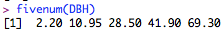
\includegraphics[keepaspectratio=true, scale=0.75]{ch1_56_fivenum.png}\\

\textbf{b.} Make a box plot:\\
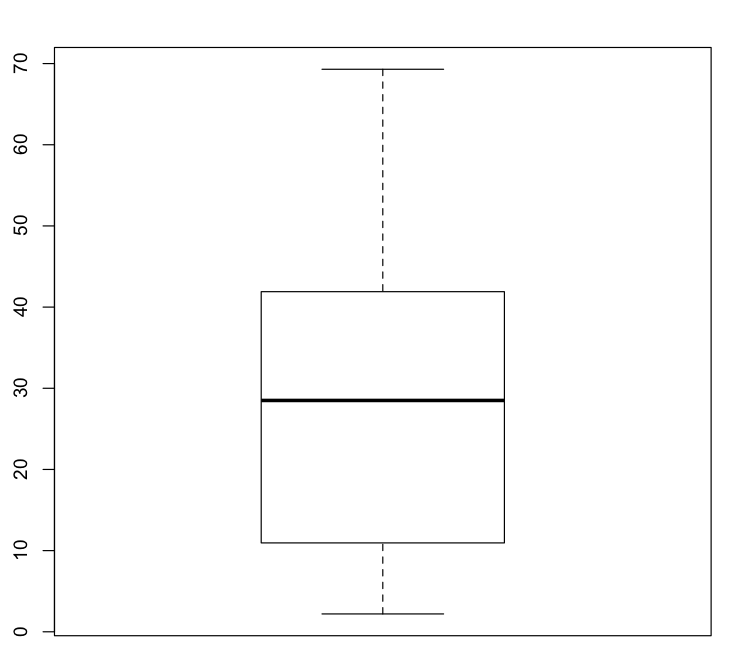
\includegraphics[keepaspectratio=true, scale=0.2]{ch1_56_boxplot.png}\\

\textbf{c.} Make a histogram:\\
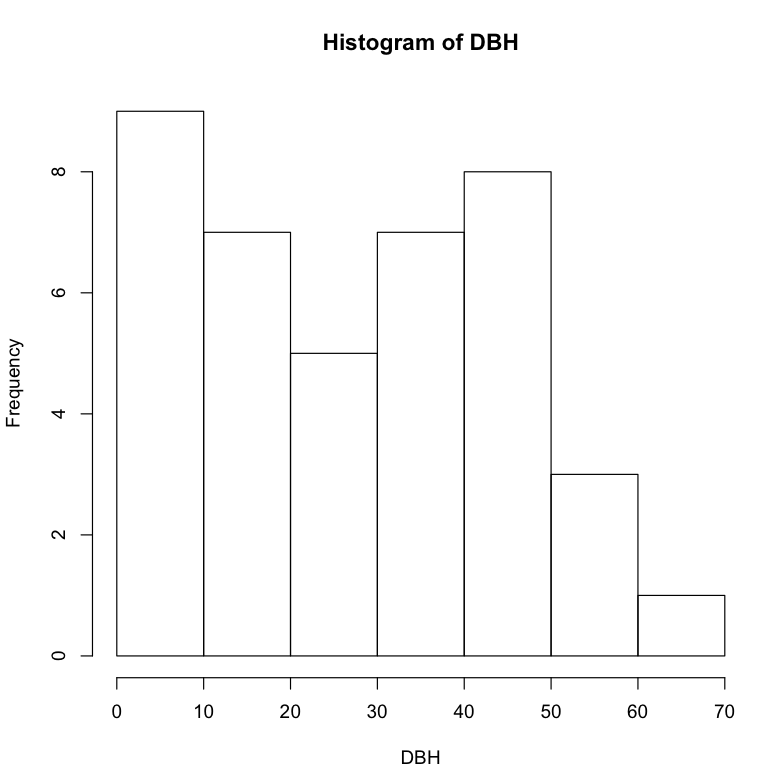
\includegraphics[keepaspectratio=true, scale=0.2]{ch1_56_histogram.png}\\

\textbf{d.} Write a short summary of the major features of the distribution:\\

The distribution seems to have many values on the at the low end and the numbers decrease towards the higher end (I guess this is called left skewed?). I prefer the histogram since I am used to them, and am very inexperienced with boxplots.\\

\textbf{64)} Analyze the CO2 data:\\

\textbf{a.} Find the five number summary:\\
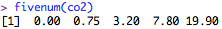
\includegraphics[keepaspectratio=true, scale=0.75]{ch1_64_fivenum.png}\\
This summary suggests that the distribution is right skewed because the distance between the third quartile and the mean is much greater than the distance between the first quartile and the mean.\\

\textbf{b.} What are the outliers. Make a histogram. Do you agree with the suspected outliers?:\\
The IQR is 7.05, and $Q_3$ is 7.80 so any values above 14.85 are suspected outliers. These are Australia, Canada, and the United States.\\
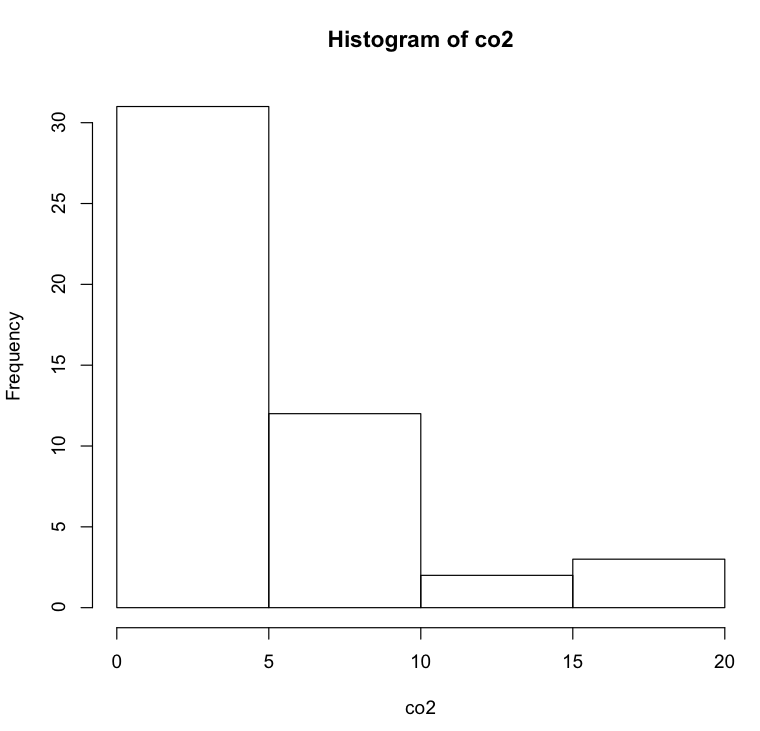
\includegraphics[keepaspectratio=true, scale=0.2]{ch1_64_histogram.png}\\
I agree with the suspected outliers, since according to my knowledge of statistics that is what is correct.\\

\textbf{66)} Analyze oil data.\\

\textbf{a.} Find the mean and median. Explain how their relationship shapes the distribution:\\
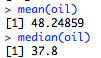
\includegraphics[keepaspectratio=true, scale=0.7]{ch1_66_meandian.png}\\
The median being lower than the mean implies that most of the values are below the mean. This means the distribution is skewed towards the left.\\

\textbf{b.} Give the five number summary and explain how it reflects the shape of the distribution:\\
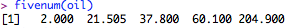
\includegraphics[keepaspectratio=true, scale=0.75]{ch1_66_fivenum.png}\\
The mean is closer to the first quartile than the third, which reflects a leftward skew. Also the very high maximum displays that there is a small number of extremely high values.\\

\textbf{70)} Calculate the mean and standard deviation for the following metabollic rates: 1792 1666 1362 1614 1460 1867 1439\\
The mean is calculated by simply summing the values and dividing by the number of how many there are (here 7). The mean here is 1600. The deviations are found by subtracting the mean from each value:
\begin{align*}
1792 - 1600 = 192 &\rightarrow (1792 - 1600)^2 = 36864\\
1666 - 1600 = 66 &\rightarrow (1666 - 1600)^2 = 4356\\
1362 - 1600 = -238 &\rightarrow (1362 - 1600)^2 = 56644\\
1614 - 1600 = 14 &\rightarrow (1614 - 1600)^2 = 196\\
1460 - 1600 = -140 &\rightarrow (1460 - 1600)^2 = 19600\\
1867 - 1600 = 267 &\rightarrow (1867 - 1600)^2 = 71289\\
1439 - 1600 = -161 &\rightarrow (1439 - 1600)^2 = 25921
\end{align*}
Note that the sum of the deviations (the unsquared value) is 0. Since we are trying to get some sort of a feel for an average \"error\" from the mean, we square the values to prevent this. Now we get the variance by simply dividing the sum of the squared deviations by $n-1$, so here by 6. This gives a variance of $$\sigma^2 = 5968.61$$ Now to get the standard deviation we take the square root to give $$ \sigma = 77.25 $$.\\

\textbf{88)} Show that the average distance from the mean of a value $x$, ($x_i-\bar{x}$), is always 0:\\
Consider a number of values $x$. The mean of these values, $\bar{x}$, is the sum of them all divided by the number of them, $n$. The sum of their deviations is $x_i - \bar{x}$
where $x_i$ is the $i^{th}$ value. Adding these looks like this:
\begin{align*}
  (x_0 - \frac{\Sigma x_i}{n}) + (x_1 - \frac{\Sigma x_i}{n}) + ... + (x_n - \frac{\Sigma x_i}{n}) &= \Sigma x_i - n\left(\frac{\Sigma x_i}{n}\right)\\
  &= \Sigma x_i - \Sigma x_i\\
  &= 0
\end{align*}
\end{document}
